\chapter{Pose Error Estimation}
\label{chap4}

\section{Introduction}

The main objective of this project is to determine a quadcopter's pose estimation accuracy as given by its on-board sensor suite. Here, the pose refers to a six-dimensional vector describing an object's position and angular orientation. The pose estimation accuracy must be performed in the outdoors to allow the quadcopter access to its global positioning sensor (GPS). To this end, a computer vision pose measurement system (CVS), which extracts six-dimensional pose data from a calibration object in the system's view, was designed and implemented. However, before the CVS could be used to make pose measurements, its measurement accuracy first needed to be determined. 

In Chapter~\ref{chap3} it was found that the pose measurement error of the CVS has high interdimensional dependence, as demonstrated by the covariance matrix of the CVS's measurement error data in Equation~\ref{eq:covariance-matrix} and the contour plots in Figure~\ref{fig:err-contour}, meaning that the CVS's pose measurements and correseponding measurement errors are constantly changing, varying with the calibration board's current pose relative to the CVS's camera. Also, despite using the RANSAC algorithm to filter out any outlier data points, the pose measurement data is still fairly complex and noisy.

In the context of this project, it is important to know what the accuracy of a pose measurement sample is to ensure that it is more accurate than the pose estimate from the quadcopter. This makes it necessary to be able to determine the measurement error of any arbitrary pose measurement sample of the CVS.\@ It was decided that a machine learning method will be employed to accomplish this. Machine learning is where a computer model is trained to recognise patterns within a set of input data and output information on the patterns which are of interest to the machine learning model's designer. 

This chapter sets out to explain the process behind making a machine learning model that can estimate, within reasonable accuracy, what the pose measurement error of the CVS is for any arbitrary input measurement vector. It starts off with some background information on the model selection, design and training. The validation phase of the trained model is then discussed and the accuracy of the final model is presented, followed by a brief discussion on it. 

\section{Model Design}

\subsection{Introduction}

This section discusses the design aspects of the machine learning model. It begins with giving some background information on the processes involved in designing a model, including model selection, training and validation. These individual aspects are then discussed in more detail. 

\subsection{Background}

Designing a machine learning model can consist of three basic steps. These steps are listed as follows:

\begin{enumerate}
  \item Select machine learning model type.
  \item Train the model.
  \item Validate the trained model's accuracy. 
\end{enumerate}

First, the model type is selected. As stated previously, the CVS's pose measurement data is fairly complex, interdimensionally dependant and is high dimensional. A neural network model was therefore selected as a machine learning model basis. It has previously been shown by~\cite{tu1996advantages} that neural networks excel at handling complicated data and detecting and extracting complex, non-linear relationships within the input data. Furthermore, the radial basis neural network (RBFNN) was selected as the neural network topology. RBFNN's provide superior results when compared to traditional feed-forward networks, when noisy data sets are used, as proven by~\cite{xie2011comparison}. The data is not time dependant, making the recurrent neural network topology unnecessarily complex for this application.  

Next, model training takes place. Here, the network is trained to take an input and adjust is internal weights in such a way that the input data is best translated to the desired output by using a supervised training scheme, such as the backpropagation procedure. In this case, the network input would be the six-dimensional pose vector produced by the CVS and the network output is the corresponding measurement error of the input pose vectors.  

Finally, to test and validate the accuracy of the trained model, it is tested with another set of input pose data of which the measurement error is already known. This data set can then be used to select and refine the training parameters of the network model. 

The design process is iterative, where steps 2 and 3, and perhaps 1, can be repeated until a model which outputs satisfactory results is produced. 

\subsection{Model Training}

Training a machine learning model is perhaps the most crucial aspect of the model design phase. Here, the hidden layer and nodes of the RBFNN's are initialised and assigned a initial weighting factor. The model is then adjusten and optimised through a supervised training method called backprogagation, demonstrated in Figure~\ref{fig:chap4-backprogagation}.

\begin{figure}
  \centering
  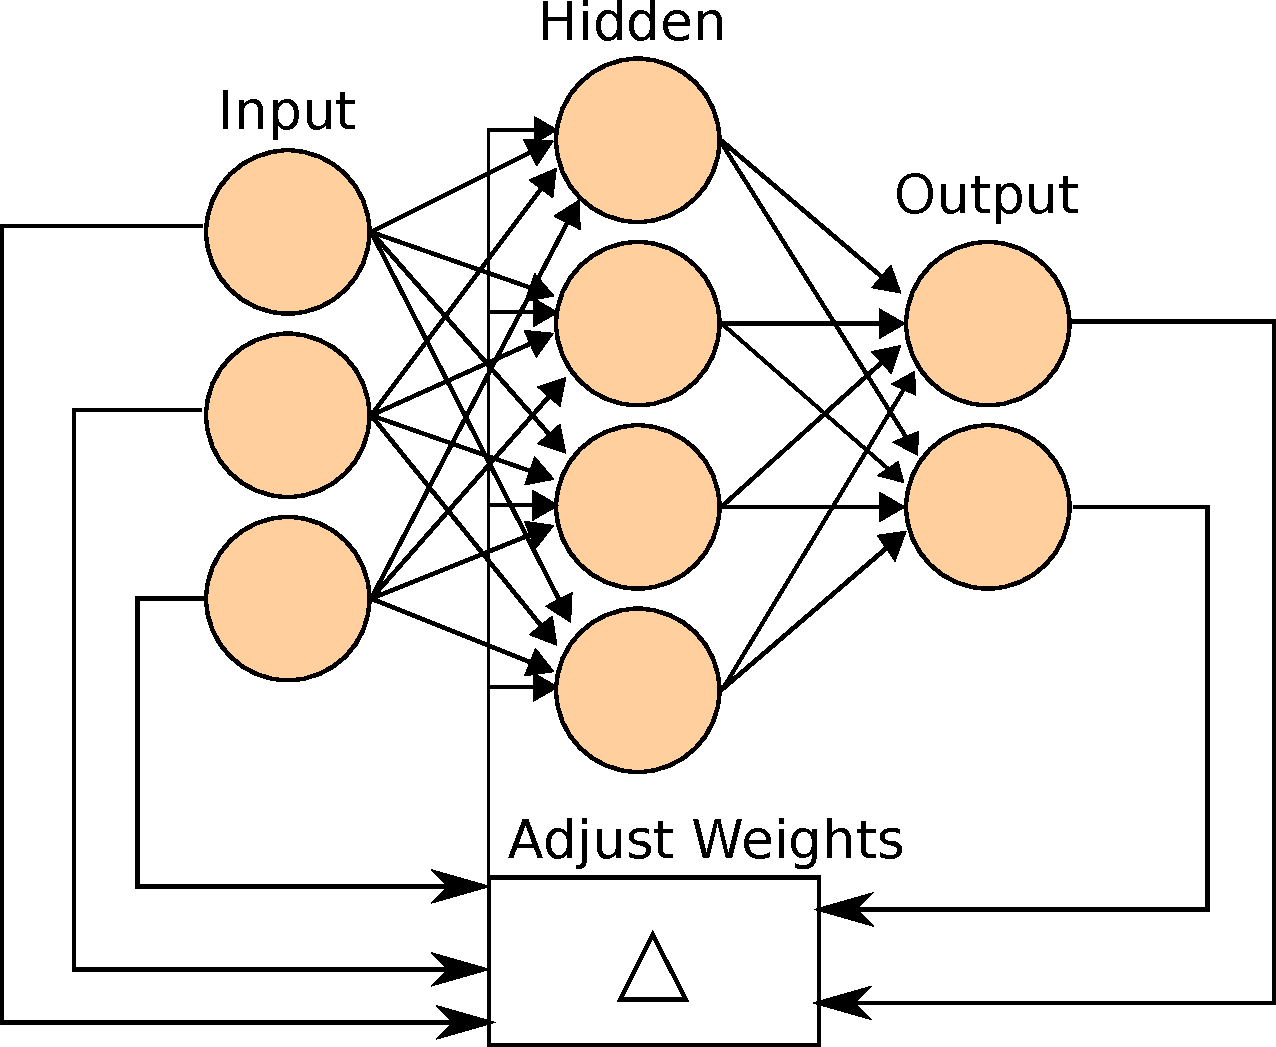
\includegraphics[width=0.5\textwidth]{figures/chapter4/backpropagation}
  \caption[A neural network implementing the backpropagation procedure.]{A figure of a neural network implementing the backpropagation procedure. Adapted from~\cite{ann-wiki-pic}.}
\label{fig:chap4-backprogagation}
\end{figure}

The backpropagation method works as follows. The hidden nodes are initialised with an initial weighting factor. The input training data is then fed to the network and its output is then compared to the training set's output data. Based on this difference, the hidden nodes' weighting factors are adjusted in an attempt to minimise the difference. Then, the input data is fed to the adjusted network again and its new output is compared to the output training data, where the weights are adjusted again. This process is repeated until the mean square error of the output's deviation from the training data falls below a set threshold or converges to zero. 

Factors that will affect the network's accuracy, are the number of nodes in the hidden layer as well as the strictness of fit that the designer selects. The number of hidden nodes is a measure of the complexity of the data it can process and also reflects the network's own complexity. However, when too many nodes are selected, there is a significant risk that the model will capture and attempt to model the noise and outlier data in a data set, instead of only characterising the underlying relationships between the input and output. This phenomenon is known as overfitting and can be observed when a model with a very small training error is exposed to new input data and the error is a few orders of magnitude larger than for the training data. Here, the model describes the training data set very well, but any data set that is not very similar to the training data set will be handled very poorly. This is why the model validation phase is a very important aspect of model training, to ensure that overfitting does not take place. 

The strictness of fit measure determines to what extent the model will attempt to fit itself to the training data. This parameter is important, since neglecting to replicate the training data adequately defeats the purpose of training the model to fit the data in the first place. However, if this parameter is too strict, the model will attempt to model the outlier and noisy data points as well, which is very undesirable. Therefore, a fine balance needs to be found for the strictness of fit and the number of hidden nodes to produce a satisfactory network.  

To train the model for this project, two sets of data were used, one for training and another for model validation. Both of these data sets were taken from the data sets generated during the Vicon measurement test, where the measurement accuracy of the CVS was determined by comparing its measurements to that of the measurements made by a Vicon system. It includes both the pose data from the CVS and its corresponding measurement error. It was decided to use 300 training samples, giving 50 samples per dimension for training. The training data was selected to be uniformly distributed to place equal importance on the entire measurement spectrum. The uniformity of the data in each dimension was checked with the Chi-square ($\chi^2$) goodness-of-fit test, with the hypothesis being that the set is uniformly distributed. As a rule of thumb, if the P-value for the $\chi^2$ test falls below 5\%, then the hypothesis is statistically insignificant and must therefore be rejected. The training data was selected in such a way that the P-value does not fall below 45\% for the data in each dimension. Furthermore, the input and output training data sets were normalised to a range of $[-1, 1]$, since the pose vector contains different measurement units (degrees and metres). All subsequent inputs to and outputs from the network must be normalised and denormalised with the same values that the training data was normalised with.  

Matlab's\footnote{Matlab v8.4.0.150421 (R2014)} Neural Network toolbox\footnote{Neural Network Toolbox v8.2.1} was used to train the RBFNN and get the output for subsequent input data. The function prototype is given by 

\begin{center}
  \verb|net = newrb(P,T,goal,spread,MN,DF)|
\end{center}

Here, $P$ and $T$ are the $300\times6$ input and output training data matrices. The \emph{goal} parameter is the error threshold for the training data and \emph{spread} is the strictness of fit parameter, while $\mathit{MN}$ and $\mathit{DF}$ define the maximum number of hidden nodes and dictate the amount of nodes to increase by between each training iteration. Adjusting the \emph{spread} and $\mathit{MN}$ parameters are the primary ways of manipulating the network to produce more accurate outputs. 

\subsection{Model Validation}

A model validation procedure is used to ensure that the RBFNN has been properly trained and that overfitting did not occur during training. The validation data set comes from the same Vicon test the training data comes from. Another 300 pose measurement samples were used for the validation data set and they were selected at random. Therefore, given that the training data is uniformly distributed, the validation set should fall within the training data. Figure~\ref{fig:chap4-scatter-tr-v} displays the scatter plots for the translation and rotation vectors for the training and validation sets and shows that they indeed to overlap to a large degree. 

\begin{figure*}
  \centering
  \begin{subfigure}{\textwidth}
    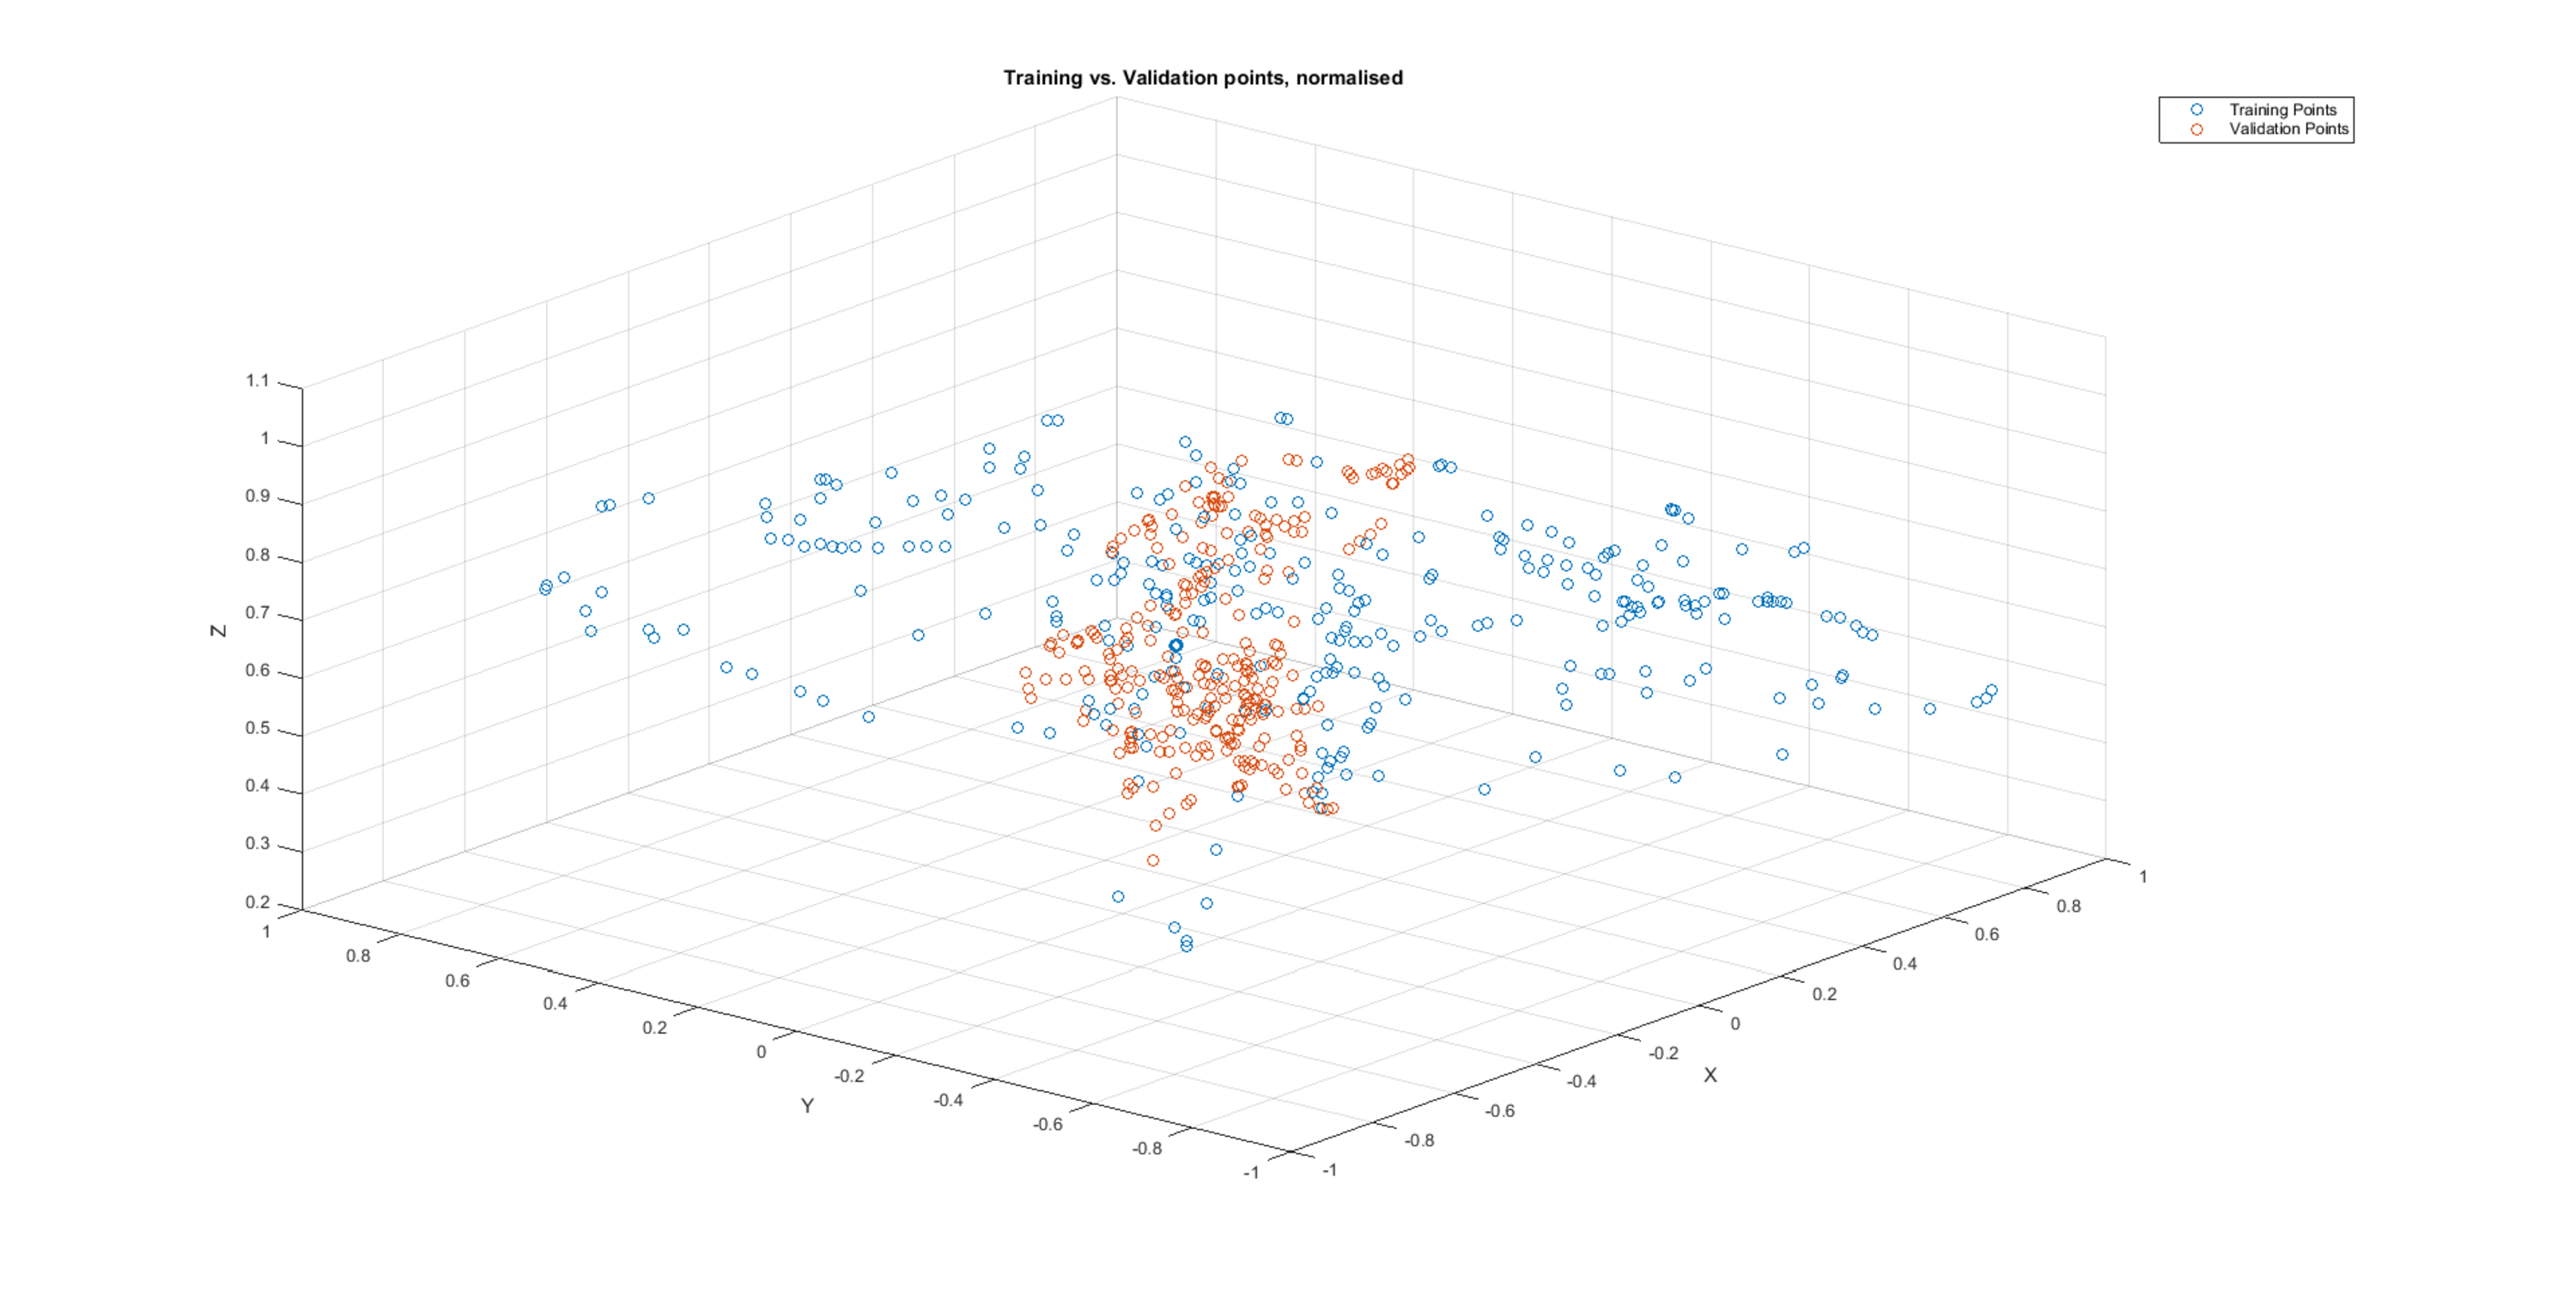
\includegraphics[clip, trim = 100 50 100 0, width=\textwidth]{figures/chapter4/3d_pose_tr_v}
    \caption{}
  \end{subfigure}
~
  \begin{subfigure}{\textwidth}
    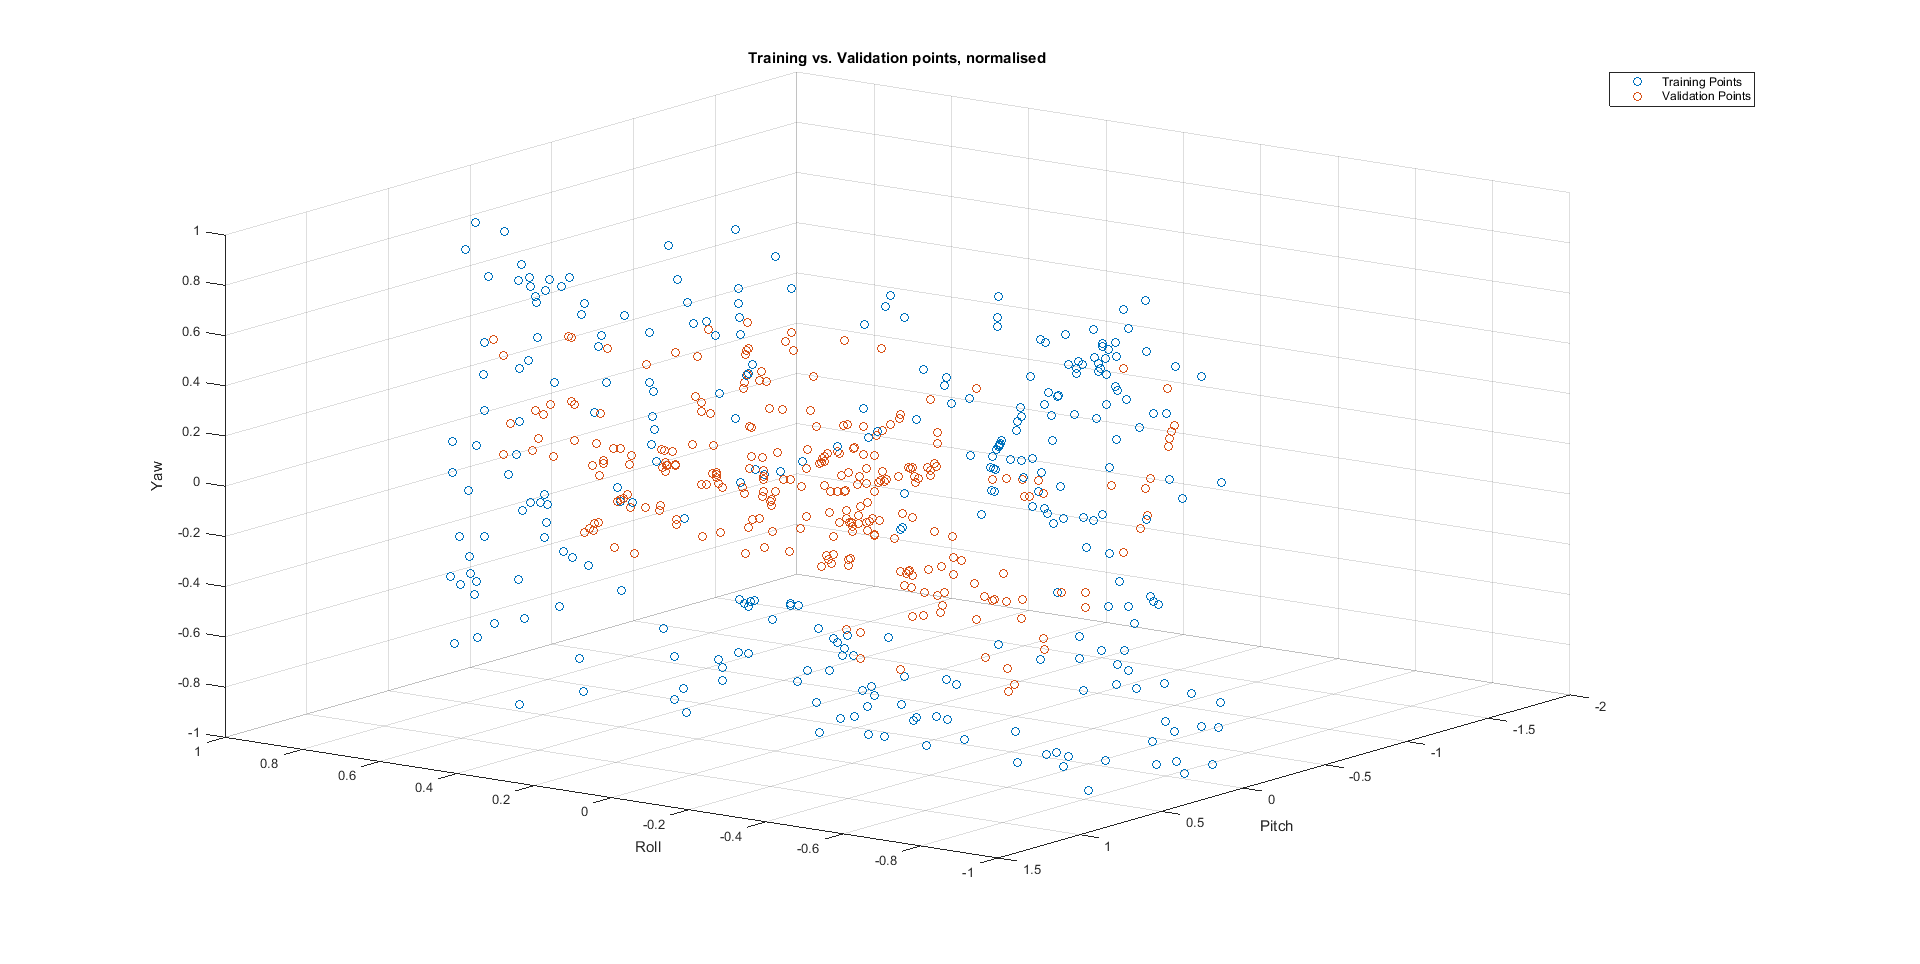
\includegraphics[clip, trim = 100 50 100 0, width=\textwidth]{figures/chapter4/3d_rot_tr_v}
    \caption{}
  \end{subfigure}
  \caption[Scatter plots of the training and validation data. ]{Normalised scatter plots of the translation and rotation data points for the training and validation data sets. }
  \label{fig:chap4-scatter-tr-v}
\end{figure*}

The error was determined by feeding the validation input data into the trained network and comparing its output with the validation error data. The mean square error was used as a measure of accuracy. This set was used to adjust the \emph{spread} and $\mathit{MN}$ training parameters, where the best combination would produce the smallest training and validation mean square errors. 

\section{Results}

With the training and validation data sets selected, the model design could begin. Different combinations of training parameters for the \verb|newrb| Matlab function were tested. It was found that the \emph{spread} parameter played the largest part in the mean square error during training and validation. This may be because the input data changes relatively quickly and contains a fair amount of noise. It was found that forcing the RBFNN to go through all the points caused the mean square error to rise when it was tested with the validation set, indicating that the model was being overfitted. It was therefore decided to keep the spread parameter small to allow the RBFNN to ignore what it classifies as outlier data and rather describe the general trend in the data. 

Furthermore, changing the maximum number of hidden nodes also influenced the accuracy of the network. Leaving the $MN$ parameter to its default will let the maximum number of hidden nodes go up to the number of training samples, 300 nodes in this case, making the network overly complex and slow. It was found that the network is more accurate with both the training and validation data sets when the hidden nodes number only about 10\% of the number of samples. 

A training parameter combination that was found to work well, was network with a \emph{spread} of 8\e{-1} and 8 hidden nodes. This combination gives a normalised mean square error of approximately 1.9\e{-2} with the validation data set, and 5.1\e{-3} with the training set, whereas the default values of 1 and 300 gives a mean square error of 3.14\e{4} and 7.1\e{-5} for the validation and training sets respectively. The results with the 300 hidden nodes demonstrates the effect of overfitting well: the training set produces very small errors, but gives a very large deviation when used with a validation data set.    

Figure~\ref{fig:chap4-rbf-train} shows results of the RBFNN model when tested with the training data set. It can be seen that the model's estimate very closely resembles the training set's error, indicating that the model is well-trained. 

\begin{figure*}
  \begin{subfigure}{0.3\textwidth}
    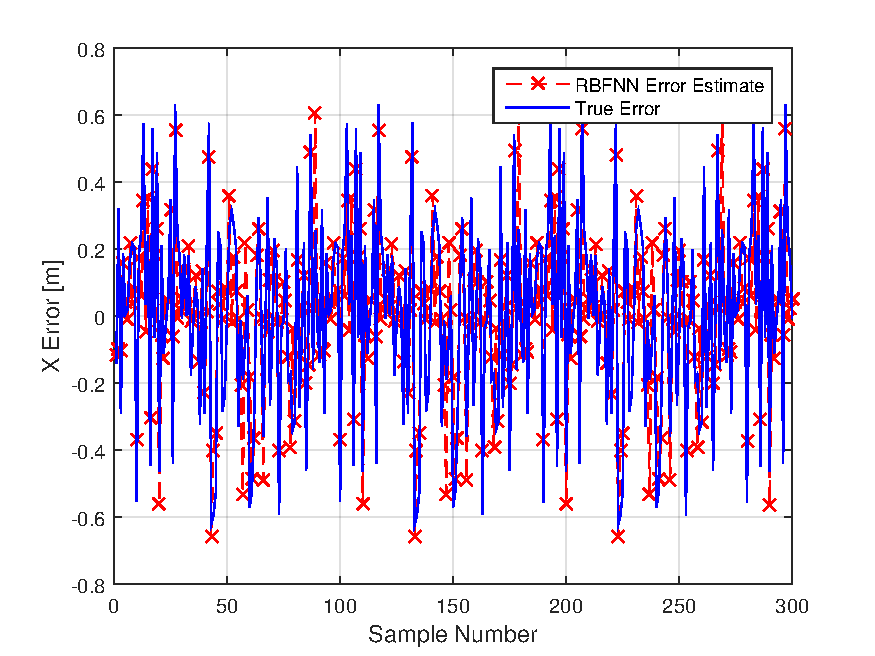
\includegraphics[width=\textwidth]{figures/chapter4/x_train}
    \caption{}
  \end{subfigure}
~
  \begin{subfigure}{0.3\textwidth}
    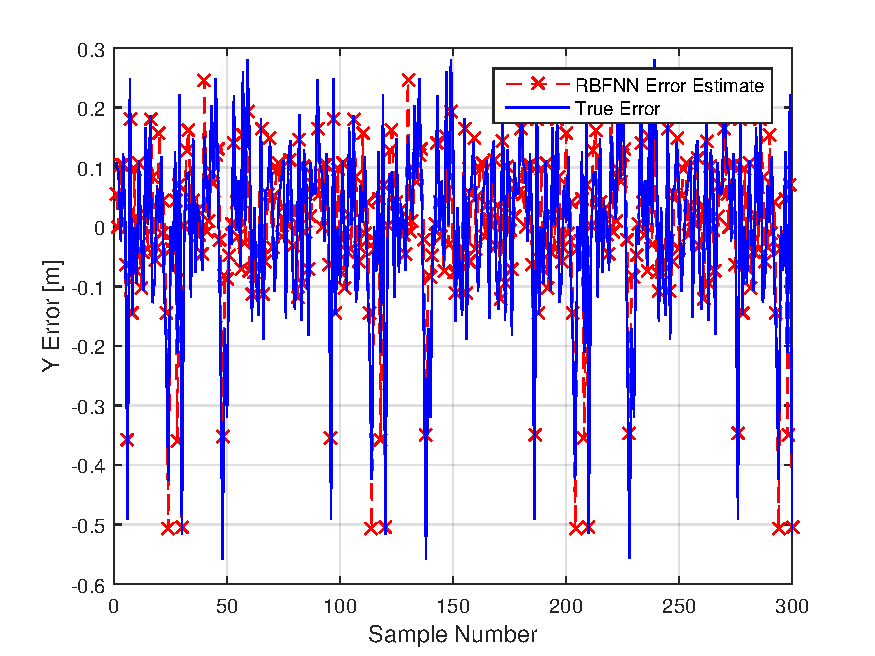
\includegraphics[width=\textwidth]{figures/chapter4/y_train}
    \caption{}
  \end{subfigure}
~
  \begin{subfigure}{0.3\textwidth}
    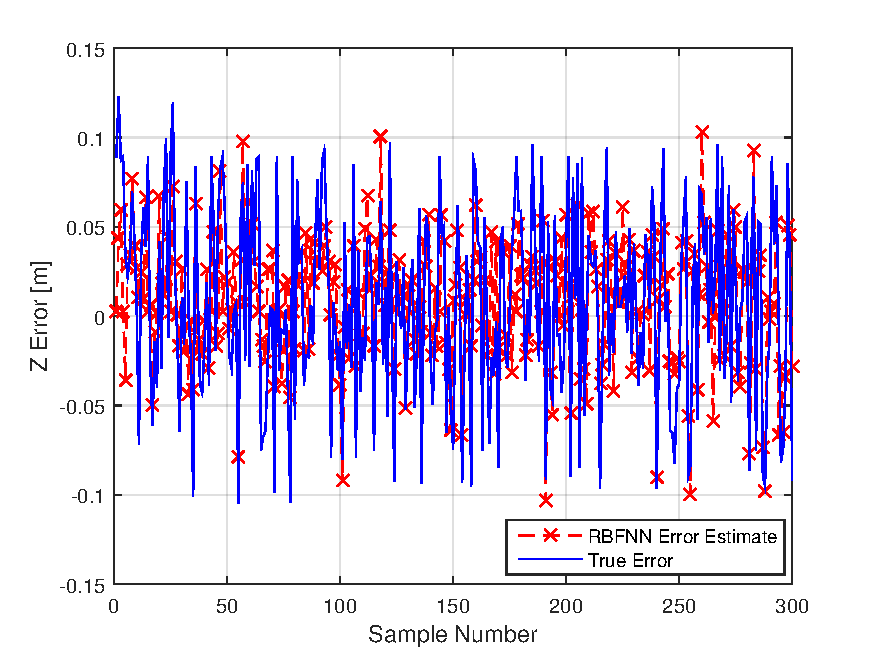
\includegraphics[width=\textwidth]{figures/chapter4/z_train}
    \caption{}
  \end{subfigure}

  \begin{subfigure}{0.3\textwidth}
    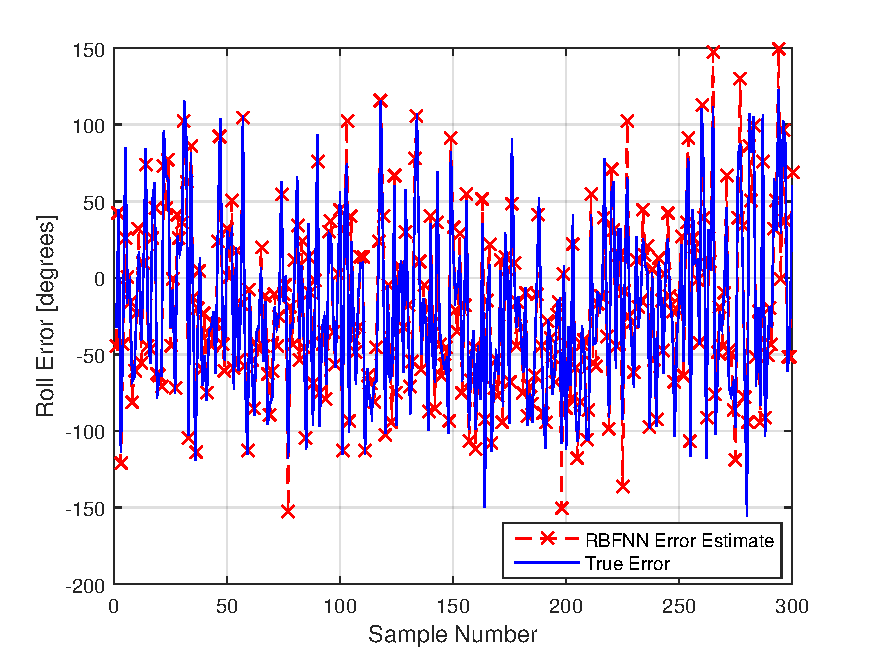
\includegraphics[width=\textwidth]{figures/chapter4/roll_train}
    \caption{}
  \end{subfigure}
~
  \begin{subfigure}{0.3\textwidth}
    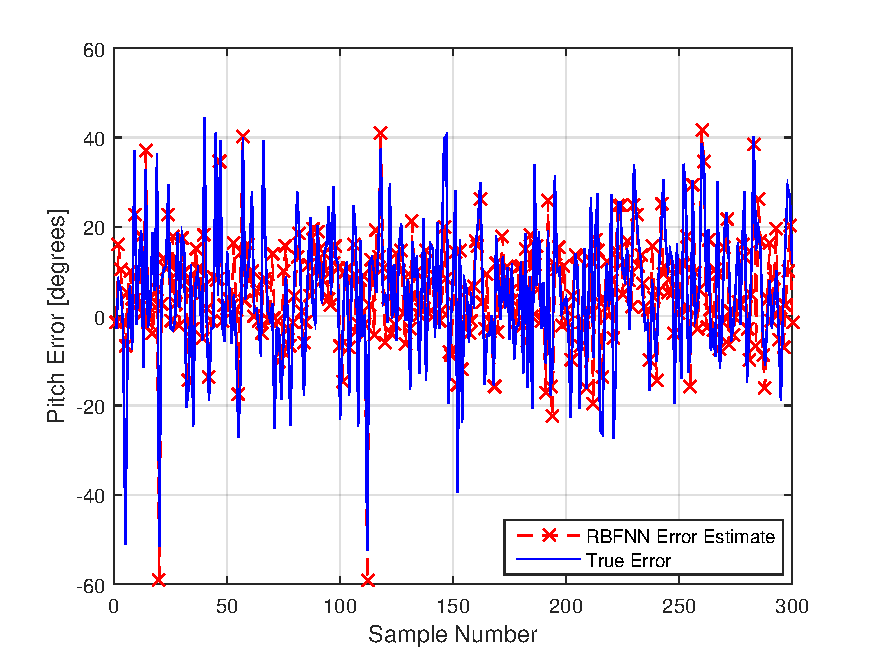
\includegraphics[width=\textwidth]{figures/chapter4/pitch_train}
    \caption{}
  \end{subfigure}
~
  \begin{subfigure}{0.3\textwidth}
    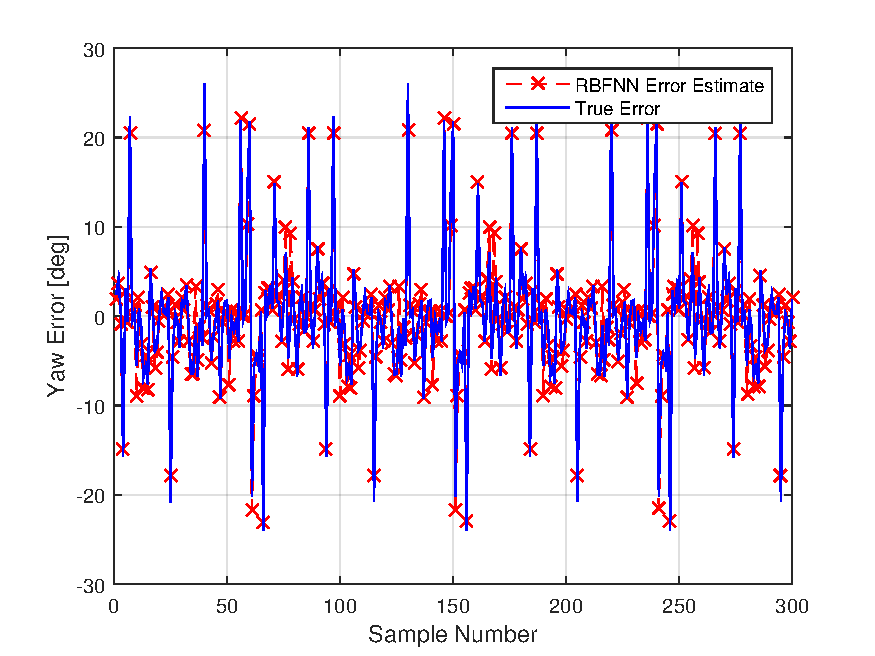
\includegraphics[width=\textwidth]{figures/chapter4/yaw_train}
    \caption{}
  \end{subfigure}
  \caption[The output of the RBFNN when used with the training set input.]{A plot of the output of the RBFNN for the different dimensions when used with the training data set.}
  \label{fig:chap4-rbf-train}
\end{figure*}

Figure~\ref{fig:chap4-rbf-valid} shows the model's output when tested with the validation data set. Here it can be seen that the RBFNN's error estimate deviates somewhat from the true error, however it follows the general trend in the data and ignores the noisy outlier data spikes. Furthermore, it generally gives an overly conservative estimate, often overestimating the error for a pose vector. This is not ideal, but is safer than underestimating the error. In general, the translation dimensions are fairly accurate. However, with the exception of the pitch dimension, the angular orientation dimensions show significant deviations from the true error, deviating up to $\ang{80}$ from the true error. 

\begin{figure*}
  \begin{subfigure}{0.3\textwidth}
    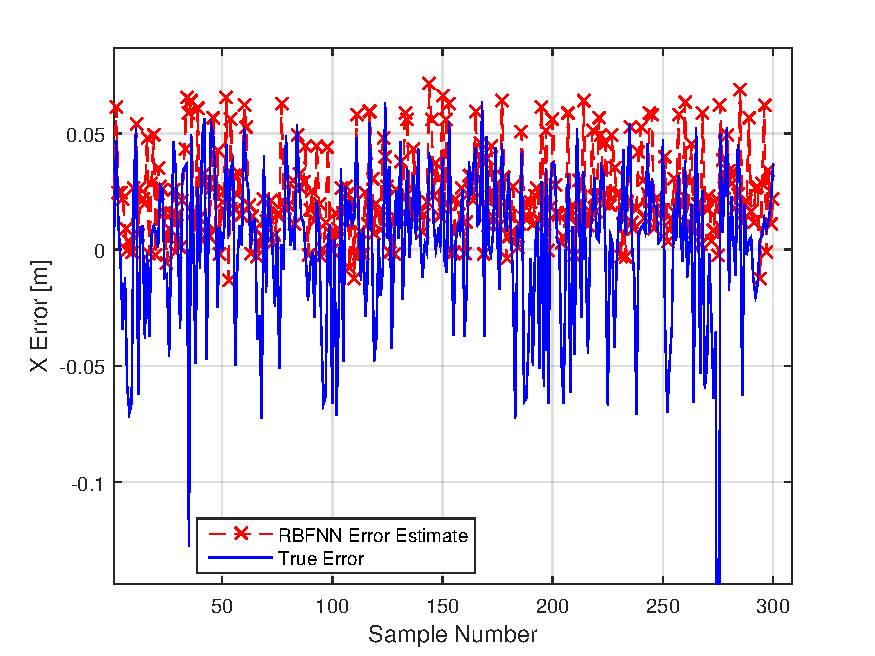
\includegraphics[width=\textwidth]{figures/chapter4/x_valid}
    \caption{}
  \end{subfigure}
~
  \begin{subfigure}{0.3\textwidth}
    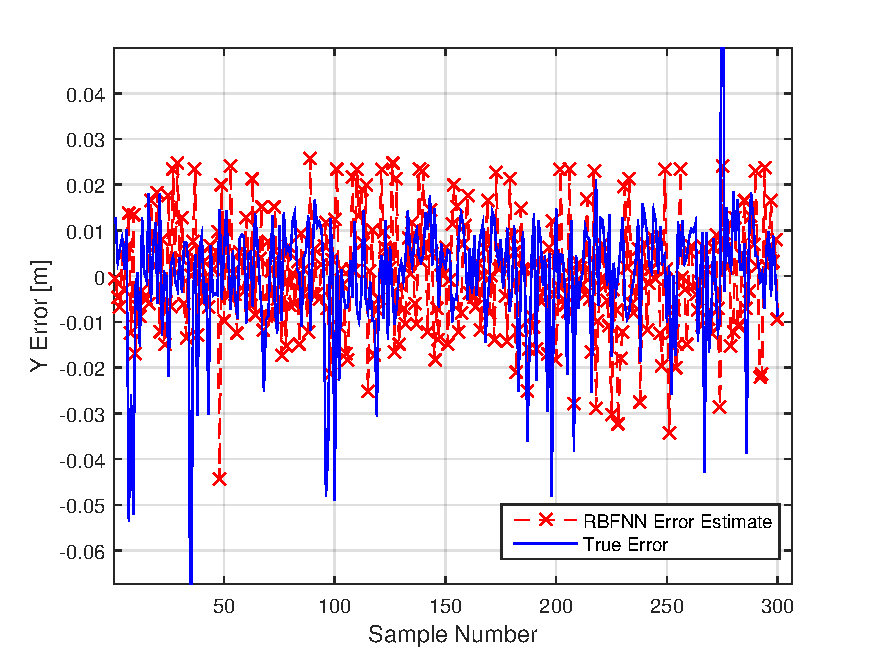
\includegraphics[width=\textwidth]{figures/chapter4/y_valid}
    \caption{}
  \end{subfigure}
~
  \begin{subfigure}{0.3\textwidth}
    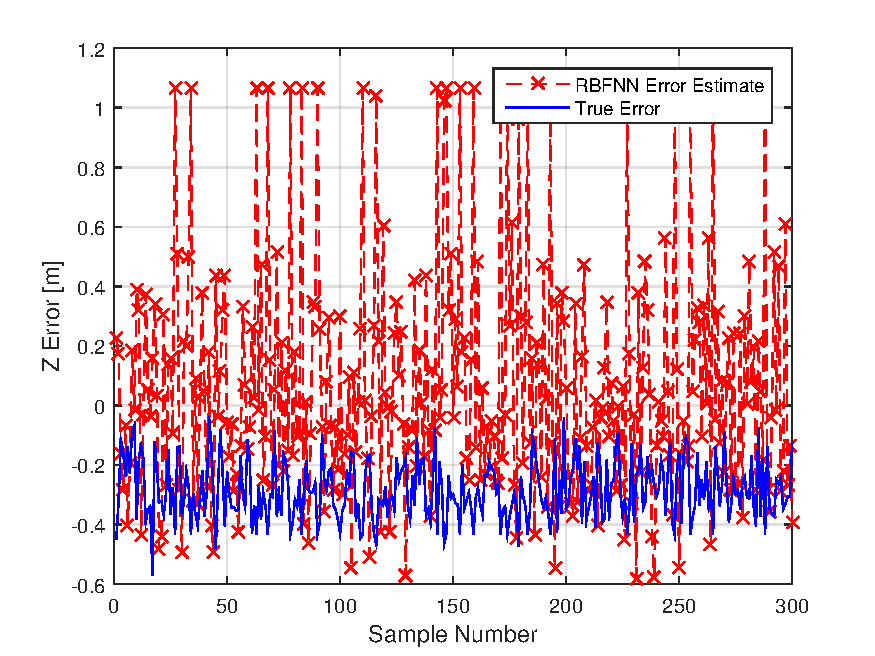
\includegraphics[width=\textwidth]{figures/chapter4/z_valid}
    \caption{}
  \end{subfigure}

  \begin{subfigure}{0.3\textwidth}
    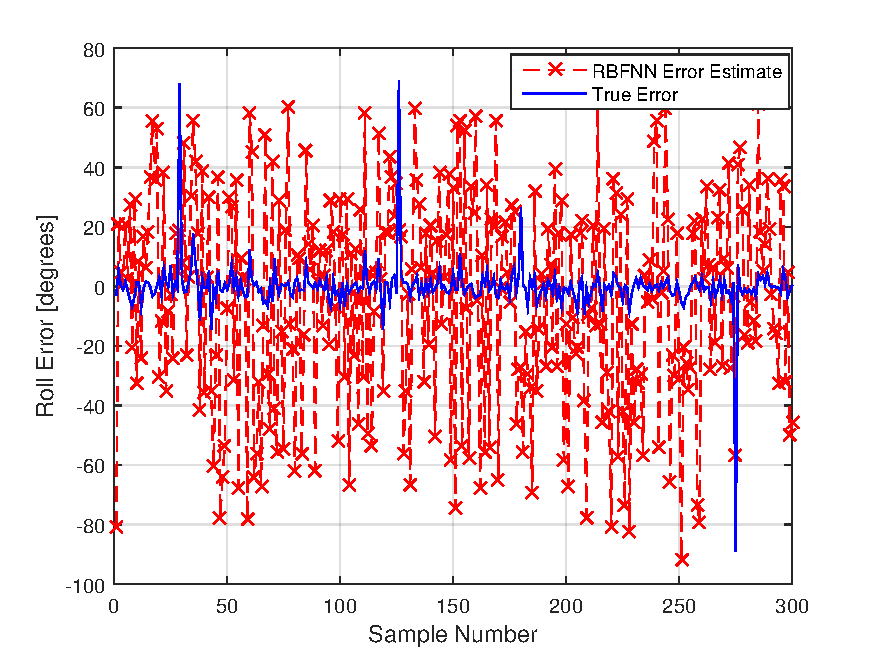
\includegraphics[width=\textwidth]{figures/chapter4/roll_valid}
    \caption{}
  \end{subfigure}
~
  \begin{subfigure}{0.3\textwidth}
    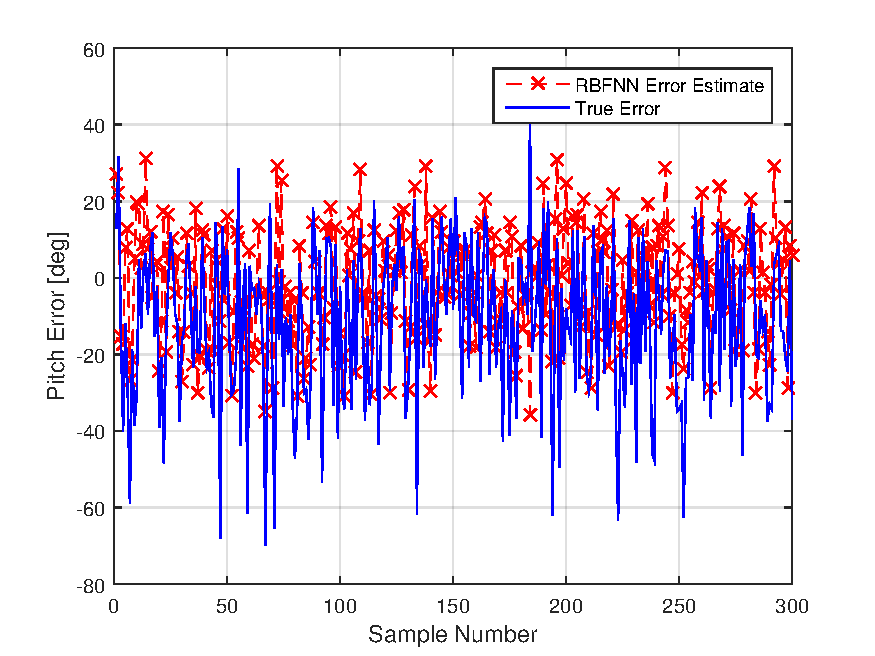
\includegraphics[width=\textwidth]{figures/chapter4/pitch_valid}
    \caption{}
  \end{subfigure}
~
  \begin{subfigure}{0.3\textwidth}
    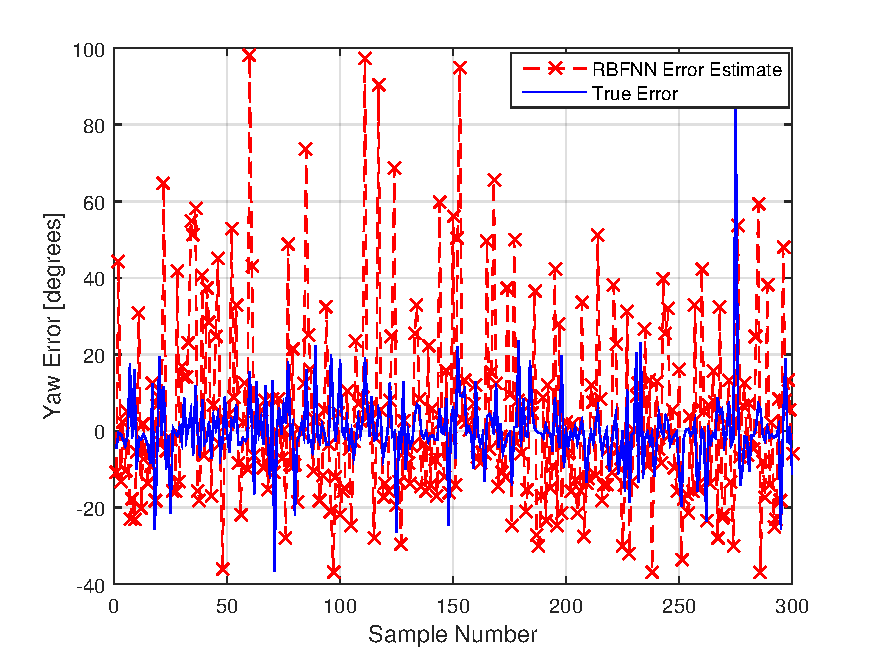
\includegraphics[width=\textwidth]{figures/chapter4/yaw_valid}
    \caption{}
  \end{subfigure}
  \caption[The output of the RBFNN with the validation set input.]{A plot of the output for the different dimensions of the RBFNN when used with the validation data set.}
  \label{fig:chap4-rbf-valid}
\end{figure*}

\section{Conclusion}

In this chapter, a machine learning model was designed to model and predict the complex and dimensionally dependant pose measurement error of the CVS.\@ A radial basis function neural network was selected to do this: it takes a six-dimensional pose measurement vector from the CVS and outputs the corresponding measurement error for the input sample. The network was trained and validated by two different data sets from the same measurement test and produces a mean square error of 1.9\e{-2} for the validation set, indicating a good model fit for the data. 

The trained network is now ready to predict the measurement error for the CVS with pose measurement data generated by a quadcopter in flight. This data can then be used to determine the pose estimation accuracy of a drone in flight. 
